\documentclass[11pt]{article}
\usepackage[margin=1in]{geometry}
\usepackage{fancyhdr}
\usepackage{enumitem}
\usepackage{parskip}
\usepackage{xcolor}
\usepackage{graphicx}

% Personal notes: \comment{Write your thoughts here.}
% Notes appear in grey in the compiled document; blank lines are supported.
\definecolor{commentgray}{gray}{0.5}
\newcommand{\comment}[1]{{\color{commentgray}#1}}

\pagestyle{fancy}
\fancyhf{}
\fancyhead[C]{\textbf{SEG2105}}
\fancyfoot[C]{\thepage}

\newcounter{chapterNumber}
\setcounter{chapterNumber}{6}
\newcounter{headerOneCount}
\newcounter{headerTwoCount}[headerOneCount]
\setcounter{headerOneCount}{-1}
\renewcommand{\theheaderOneCount}{\arabic{headerOneCount}}
\renewcommand{\theheaderTwoCount}{\arabic{headerTwoCount}}

\newcommand{\Title}[1]{%
  \begin{center}
    \fontsize{24}{28}\selectfont\textbf{#1}
  \end{center}
  \vspace{1em}
}

\newcommand{\HeaderOne}[1]{%
  \refstepcounter{headerOneCount}%
  \setcounter{headerTwoCount}{-1}%
  \vspace{0.75em}
  \noindent\fontsize{18}{22}\selectfont\textbf{\arabic{chapterNumber}.\theheaderOneCount\ #1}\par
  \vspace{0.5em}
}

\newcommand{\HeaderTwo}[1]{%
  \refstepcounter{headerTwoCount}%
  \vspace{0.5em}
  \noindent\fontsize{16}{20}\selectfont\textbf{\arabic{chapterNumber}.\theheaderOneCount.\theheaderTwoCount\ #1}\par
  \vspace{0.4em}
}

\newcommand{\BodyText}[1]{%
  \fontsize{12}{15}\selectfont #1\par
}

\newcommand{\Question}[1]{%
  \fontsize{15}{15}\selectfont #1\par
}

\newenvironment{NumberedList}{%
  \begin{enumerate}[leftmargin=2em, itemsep=0.35em, topsep=0.35em]
}{%
  \end{enumerate}
}

\newenvironment{DottedList}{%
  \begin{itemize}[leftmargin=2em, itemsep=0.35em, topsep=0.35em, label=\textbullet]
}{%
  \end{itemize}
}



\begin{document}
\Title{Using Design Patterns}

\HeaderOne{Introduction to Patterns}
\BodyText{This is the main body text in 12pt font.}
\BodyText{The heading numbering stays consistent across the document.}

\HeaderOne{Introduction}
\BodyText{This is the main body text in 12pt font.}
\BodyText{The heading numbering stays consistent across the document.}

\HeaderOne{Abstraction-Occurence Pattern} 
\HeaderTwo{Library Example}
\BodyText{A Library book has properties such as:}
\begin{DottedList}  
  \item Title \comment{Duplicates per instance}
  \item Author
  \item Barcode \comment{Unique per instance}
\end{DottedList}
\BodyText{Each instance of the same book will have a different barcode, but title and author is the same.}
\BodyText{\textbf{How can we make a mechanism that allows us to contain unique data instead of duplicate values?}}
\BodyText{The solution lies in a one-to-many association. A single "book" instance will have many "bookItem" instances, containing a unique barcode.}

\HeaderOne{General Hiearchy Pattern}
\BodyText{}
\begin{DottedList}
  \item Context: Objects in a hierarchy can have one or more objects above them (superiors), and one or more objects below them (subordinates). Some objects cannot have any subordinates
  \item Problem: How do you represent a hierarchy of objects, in which some objects cannot have subordinates?
  \item Forces: You want a flexible way of representing the hierarchy that prevents certain objects from having subordinates. All the objects have many common properties and operation
  \item Solution:
\end{DottedList}
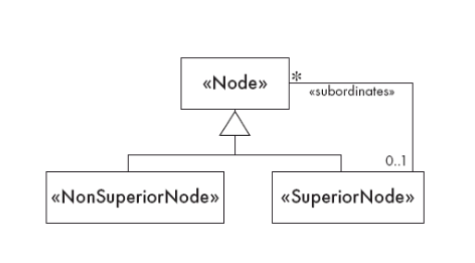
\includegraphics[width=0.5\textwidth]{Figure1.png}

\HeaderOne{Player-Role Pattern}
\BodyText{}
\begin{DottedList}
  \item Context: A role is a particular set of properties associated with an object within context. An object may play different roles in different contexts. 
  \item Problem: What is the best way to model players and roles s.t a player can change roles or have multiple roles?
  \item Forces: 
  \subitem Improve encapsulation by capturing role info
  \subitem Avoid multiple inheritance
  \subitem Instances cannot change classes 
  \item Solution:
\end{DottedList}
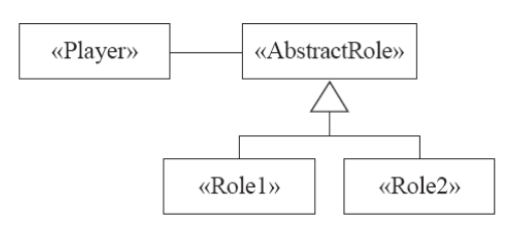
\includegraphics[width=0.5\textwidth]{Figure2.png}
\newpage
\HeaderOne{Singleton Pattern}
\BodyText{}
\begin{DottedList}
  \item Context: We need classes that only have one instance
  \item Problem: How do we ensure the impossiblity of more than one instance of a singleton class
  \item Forces: 
  \subitem Public constructors cannot ensure a single instance
  \subitem Singleton instance must also be accessible
  \item Solution: On instance, create a constructor only ONCE. Every constructor call past this will return the existing instance. 
\end{DottedList}
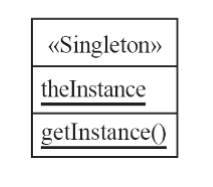
\includegraphics[width=0.5\textwidth]{Figure3.png}

\HeaderOne{Observer Pattern}
\BodyText{}
\begin{DottedList}
  \item Context: 
  \subitem Associations between classes causes classes code to be inseparable.
  \subitem Reuse of one of these classes requires the other.
  \item Problem: How do we reduce the interconnection between classes?
  \item Forces: Maximize flexibility of the system.
  \item Solution:   
\end{DottedList}

\HeaderOne{Delegation Pattern}
\BodyText{}
\begin{DottedList}
  \item Context: Another class has a method which provides a service we want to use
  \item Problem: How do we effectively make use of a method that already exists in the other class?
  \item Forces: Minimize development costs via reuse
\end{DottedList}

\HeaderOne{Facade}
\BodyText{}
\begin{DottedList}
  \item Context: Applications contain several complex packages. A programmer has to manipulate many different classes
  \item Problem: How can we simplify the view that programmers have of a complex package.
  \item Force: 
  \subitem Understanding and using an entire subsystem is hard 
  \subitem  
\end{DottedList}

\end{document}


